\documentclass{beamer}
\usetheme{utk}
\usepackage{outlines}
\usepackage{mathtools}

\title[Spectral and Hierarchical Clustering]{Spectral Clustering and Hierarchical Clustering}
\author{Roxana Barrios, Charlotte Beckford, and Sarah Harkins}
\institute{Math 526}

% Need to figure out how to set the date in the .sty document. It is inserting the current date. 


\begin{document}

\begin{frame}
\titlepage
\end{frame}

\begin{frame}
\begin{center}
  \textcolor{TennesseeOrange}{\huge Spectral Clustering}  
\end{center}

\end{frame}

\begin{frame}
\frametitle{Notation}

\begin{itemize}
    \item Let $G = (V,E)$ be an \textbf{undirected graph} with the set of vertices $V = \{ v_1, \dots v_n\}$ and the set of edges, $E$.  
    \item We will assume that $G$ is weighted with \textbf{non-negative weights} $w_{i,j}$ corresponding to the edge between the vertices $v_i$ and $v_j$. The weights are contained in the \textbf{adjacency matrix}, $W = (w_{i,j})_{i,j = 1, \dots , n}$. In an undirected graph, $w_{i,j} = w_{j,i}$. 
    \item The \textbf{degree} of a vertex $v_i$  $$d_i = \sum_{j=1}^{n} w_{i,j}$$ This forms the degree matrix $D= diag(d_1, \dots , d_n)$
\end{itemize}

\end{frame}

\begin{frame}{Problem Statement}
     You are presented with a set of $N$ data points in $d$-dimensional space and you are told to form $k$ clusters. 
\end{frame}



\begin{frame}{Algorithm}
    \begin{enumerate}
        \item Compute similarity matrix, $S \in \mathbb{R}^{nxn}$ with desired metric 
        \item \textcolor{red}{Create $W \in \mathbb{R}^{nxn}$, the weight matrix from $S$ with desired method }Form a weighted, undirected graph by constructing a similarity matrix. 
        \item Form the Laplacian matrix. 
        \item Find the eigenvectors of the Laplacian matrix associated with its $k$ smallest eigenvalues.
        %\begin{enumerate}
        %    \item This reduces the dimension of the problem: the data points are now projected into $k$-dimensional, rather than $n$-dimensional space, making clustering easier.
        %\end{enumerate}
        \item Construct a matrix whose columns house the $k$ eigenvectors found in the previous steps. Each data point is associated with a different row of the matrix. 
        \item Perform a clustering algorithm, such as $k$-means clustering, on the rows of the $n \times k$ matrix. This associates each data point with one of the $k$ clusters.
    \end{enumerate}
\end{frame}

\begin{frame}
\frametitle{Step 1: Similarity Measures}
The similarity of vertices $v_i$ and $v_j$ are given by $s_{i,j}$, which weighs the edge between those vertices. There are multiple ways to compute similarity. Here are some commonly used examples:
\vspace{0.25 cm}
\begin{outline}
    \1 Euclidean Distance
        \2 $s_{i,j} = \| v_i, v_j\|_2$
    \1 Manhattan Distance
        \2 $s_{i,j} = \sum_{i=1}^{n} | v_i - v_j|$
    \1 Gaussian Similarity Function
        \2 $s_{i,j} = exp(\| v_i, v_j\|^2 / (2\sigma^2))$
            \3 $\sigma$ control the size of the neighborhood 
\end{outline}

\end{frame}

\begin{frame}
\frametitle{Step 1: Similarity Graphs}
Once you have the similarity measurements between all pairs of vertices, there are different ways to construct the similarity graph.
\\
\vspace{0.25 cm}
Can make the algorithm more efficient by making the graph less connected, which makes its matrix representation sparse.
\vspace{0.25 cm}
\begin{outline}
    \1 $\epsilon$- neighborhood Graph
        \2 Fix $\epsilon >0$. If  $s_{i,j} > \epsilon$, then the respective nodes are considered connected. This is an unweighted graph. 
        %\2 $$
        %w_{i,j} = \begin{cases}
        %    1 & s_{i, j} > \epsilon \\
        %    0 & s_{i, j} \leq \epsilon
        %\end{cases}
        %$$
    \1 $k$- nearest Neighbor Graph
        \2 Option 1: Connect $v_i$ and $v_j$ if $v_i$ is among the $k-$nearest neighbors of $v_j$ or if $v_j$ is among the $k-$nearest neighbors of $v_i$.
        \2 Option 2: Connect $v_i$ and $v_j$ if $v_i$ is among the $k-$nearest neighbors of $v_j$ \textbf{and}  $v_j$ is among the $k-$nearest neighbors of $v_i$.
    \1 Fully Connected Graph
        \2 All vertices are connected and the edges have weights $s_{i,j}$. 
        %\2 $w_{i,j} = s_{i,j}$
\end{outline}
\end{frame}


\begin{frame}
\frametitle{Step 1: Similarity Matrices}
Represent the similarity graph as a matrix $W$. Since there are $N$ data points, $W \in \mathcal{R}^{n \times n}$, where each row and each column is associated to a particular data point (vertex).
\begin{outline}
    \1 $\epsilon$- neighborhood Graph
        %\2 Fix $\epsilon >0$. If  $s_{i,j} > \epsilon$, then the respective nodes are considered connected. This is an unweighted graph. 
        $
        w_{i,j} = \begin{cases}
            1 & s_{i, j} > \epsilon \\
            0 & s_{i, j} \leq \epsilon
        \end{cases}
        $
    \1 $k$- nearest Neighbor Graph
        %\2 Option 1: Connect $v_i$ and $v_j$ if $v_i$ is among the $k-$nearest neighbors of $v_j$ or if $v_j$ is among the $k-$nearest neighbors of $v_i$.
        %\2 Option 2: Connect $v_i$ and $v_j$ if $v_i$ is among the $k-$nearest neighbors of $v_j$ \textbf{and}  $v_j$ is among the $k-$nearest neighbors of $v_i$.
        
            $$ w_{i,j} = \begin{cases}
            s_{i,j} & v_i \textrm{ is among }k\textrm{-nearest neighbors of } v_j \textrm{ or vice versa} \\
            0 & \textrm{otherwise}
                    \end{cases}$$
              
        $$w_{i,j} = \begin{cases}
            s_{i,j} & v_i \textrm{ is among }k\textrm{-nearest neighbors of } v_j \textrm{ and vice versa} \\
            0 & \textrm{otherwise}
        \end{cases}$$
        
    \1 Fully Connected Graph \qquad $w_{i,j} = s_{i, j}$, $\forall i,j$
        %\2 All vertices are connected and the edges have weights $s_{i,j}$. 
        %\2 $w_{i,j} = s_{i,j}$
\end{outline}
\end{frame}

\begin{frame}
\frametitle{2. Graph Laplacian}
\begin{itemize}
    \item Let $D$ be the diagonal matrix with non-trivial entries 
    $$
    D_{i, i} = \sum_{j} W_{i, j}.
    $$
\end{itemize}
\begin{outline}
 \1 Unnormalized Graph Laplacian
   \2 $L = D - W$
 \1 Normalized Graph Laplacian
     \2 Random Walk
        \3 $L_{\textrm{rw}} = I - D^{-1} W$
     \2  Symmetric Matrix
        \3 $L_{\textrm{sym}} = I -D^{-1/2}WD^{1/2}$
\end{outline}
\end{frame}

\begin{frame}{3. - 5.}
    \begin{enumerate}
     \setcounter{enumi}{2}
        \item Whether you are working with $L$, $L_{\textrm{rw}}$, or $L_{\textrm{sym}}$, compute the eigenvectors
        $
        \mathbf{v}_1, \cdots, \mathbf{v}_k
        $
        associated with the $k$ smallest eigenvalues of the Laplacian matrix
        \item Construct a matrix
        $$ \textcolor{red}{X_{emb.} = }
        \begin{bmatrix}
            \mathbf{v}_1 & \cdots \mathbf{v}_k
        \end{bmatrix} \in \mathcal{R}^{N \times k}
        $$
        This step performs dimension reduction \textcolor{red}{, via spectral embedding, } because it changes the representation of the data points in $d$ dimension to points in $k$ dimensions.
    \item \textcolor{red}{Assign row $i$ of the spectral embedding, $X_{emb.}$, to be the feature vector corresponding to the vertex $v_i$. }
    \item \textcolor{red}{Perform $k$-means clustering with the feature vectors generated in the previous step.}
    \item Perform $k$-means clustering on the rows of matrix found in step 4. This assigns each row to one of $k$ clusters, and each row corresponds to a data point, so each data point is assigned to one of $k$ clusters.
    \end{enumerate}
\end{frame}

\begin{frame}{Which graph Laplacian should be used?}
To answer this question we should look at the the degree distribution of the similarity graph. 

\begin{enumerate}
    \item If the graph is very regular and most vertices
have approximately the same degree, then all the Laplacians are very similar to each other, and will
work equally well for clustering. 
\item If the degrees in the graph are very broadly distributed,
then the Laplacians differ considerably. There are several arguments that advocate for using normalized rather than unnormalized spectral clustering, and in the normalized case to use
the eigenvectors of $L_{rw}$ rather than those of $L_{sym}$.
\end{enumerate}
    
\end{frame}

\begin{frame}{Why this algorithm works}
    \begin{outline}
        \1 When clustering, you want to maximize in-cluster similarity and minimize out-cluster similarity. In terms of our similarity graphs, this is the same as finding a partition such that the edges within each group have high weight and the edges between each group have low weight.
        \1 Can address these metrics by minimizing 
        $$
        \textrm{cut}(A_1, \dots, A_k) = \frac{1}{2} \sum_{i=1}^k \, \sum_{j \in A_i, k \not \in A_k} w_{j, k}
        $$
        but in many cases the solution of this minimization problem simply separates individual vertices from the rest of the graph.
        \1 Circumvent this pitfall by explicitly requesting that the sets\textcolor{red}{, $A_i$, } are reasonably large\textcolor{red}{, via RatioCut and Ncut.}
            %\2 Unnormalized Laplacian only addresses the first metric. It work to find a partition $A_1, \dots A_k$ which minimizes
            %$$
            %\textrm{cut}(A_1, \dots, A_k) = \frac{1}{2} \sum_{i=1}^k \, \sum_{j \in A_i, k \not \in A_k} w_{j, k}
            %$$
            %\3 Becuase of this, unnormalized Laplacian may result in a partition that isolates one vertex. 
            %\2 Normalized Laplacian addresses both metrics by requesting that the sets are reasonably large.
    \end{outline}
\end{frame}

\begin{frame}{Why this algorithm works}
    \begin{outline}
    \1 One can measure the set size in terms of the number of vertices/data points it contains notated by $|A_i|$ and the weights of its edges $vol(A_i) = \sum_{j, k \in A_i} w_{j, k}$. 
    \1 Then the task is to minimize \vspace{0.1 cm}
    \begin{equation}
    RatioCut(A_1, \dots, A_k) \coloneqq \frac{1}{2}\sum_{i=1}^k \frac{1}{|A_i|}  \sum_{j \in A_i, k \not \in A_i} w_{j, k}
    \end{equation}\\ %\vspace{0.1 cm}\\
    \begin{centering}
        or
    \end{centering}
    $$
     Ncut(A_1, \dots, A_k) \coloneqq \frac{1}{2}\sum_{i=1}^k \frac{1}{vol(A_i)}  \sum_{j \in A_i, k \not \in A_i} w_{j, k}
    $$
    \end{outline}
    Spectral clustering solves relaxed versions of these problems. Relaxing the first leads to unnormalized spectral clustering and relaxing the second leads to normalized spectral clustering.
\end{frame}


\begin{frame}{Why this algorithm works}
    Can prove that (1) = $\textrm{Trace}(H'LH)$ where
    $$
    h_{i,j} = \begin{cases}
        1/\sqrt{|A_j|} &\textrm{if } v_i \in A_j \\
        0 &\textrm{else }.
    \end{cases}
    $$ The columns of $H$ are orthonormal to each other. \\
    The minimization problem is the same as 
    $$
    \min_{A_1, \dots, A_k} \textrm{Trace}(H'LH) \textrm{ subject to } H'H = I
    $$
    and spectral clustering relaxes this minimization problem to 
     $$
    \min_{M \in \mathcal{R}^{n \times k}} \textrm{Trace}(M'LM) \textrm{ subject to } M'M = I.
    $$
\end{frame}

\begin{frame}{Why this algorithm works}
    Spectral clustering is therefore solving a trace minimization problem. \\ \vspace{0.25cm}

    A version of the Rayleigh-Ritz theorem tells us that a solution is given by choosing $M$ as the matrix which contains the first $k$ eigenvectors of $L$ as columns. \\\vspace{0.25cm}

    The matrix \textcolor{red}{formed in step 4 $X_{emb.}$} is a real-valued solution matrix, but we need to convert it to a discrete partition: the standard way is to use the $k$-means algorithm (step \textcolor{red}{5}).
\end{frame}


\begin{frame}{Advantages of Spectral Clustering}
    \begin{itemize}
        \item Can be implemented efficiently even for large data sets as long as the similarity graph is sparse (uses standard linear algebra software)
        \item Makes no assumption on cluster shape or size, so particularly effective when structures of clusters are highly non-convex or when the clusters are of different densities or sizes
    \end{itemize}
    
    \begin{figure}
        \begin{minipage}[b]{0.4\textwidth}
            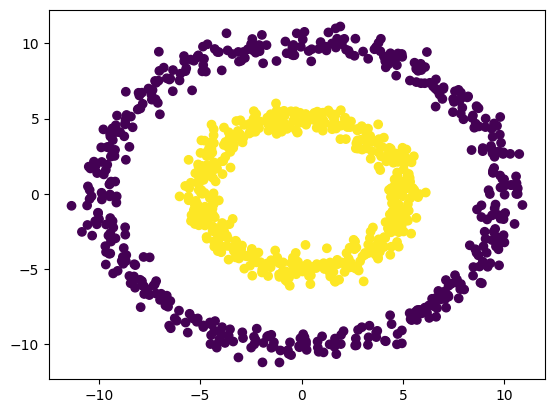
\includegraphics[width=\textwidth]{concentric_circles.png}
         \end{minipage}
        \hfill
        \begin{minipage}[b]{0.4\textwidth}
            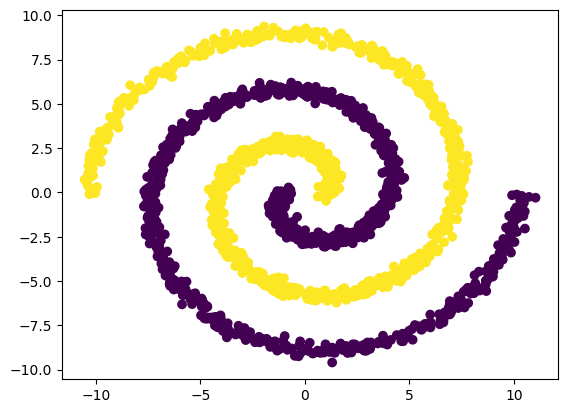
\includegraphics[width=\textwidth]{interlacing_spirals_example.png}
        \end{minipage}
    \end{figure}
\end{frame}

\begin{frame}{Disadvantages of Spectral Clustering}
    \begin{itemize}
        \item Sensitive to choice of similarity measure and its parameters, i.e. $\sigma$ in the Gaussian similarity measure
        \item The number of clusters $k$ must be pre-determined
    \end{itemize}
\end{frame}


\begin{frame}
\begin{center}
  \textcolor{TennesseeOrange}{\huge Hierarchical Clustering}  
\end{center}
\end{frame}

\begin{frame}{Overview}
\begin{outline} Start with $N$ data points.
    \1 Agglomerative Hierarchical Clustering: Create a hierarchy by first considering each individual data point to be in its own cluster and at each step merging the clusters which are most similar. Eventually, all data points will be merged into one cluster. 
    \1 Divisive Hierarchical Clustering: Create a hierarchy by first considering all data points to be in the same cluster and at each step split the farthest point in the cluster. Eventually, all data points will be isolated in their own cluster. 
\end{outline}
The order of aggregating/dividing clusters is recorded in a dendrogram, which establishes a hierarchy in which data points are most similar.
\end{frame}

\begin{frame}{Algorithm}
    \begin{enumerate}
        \item Compute the proximity matrix using a particular distance metric.
        \item Assign each data point to a cluster
        \item Merge (agglomerative) or divide (divisive) the clusters based on a chosen metric
        \item Update the proximity matrix
        \item Repeat Step 3 and Step 4 until only a single cluster remains (agglomerative) or until each data point is assigned to its own cluster (divisive)
    \end{enumerate}
\end{frame}

\begin{frame}{Step 1: Proximity Matrix} 
\begin{outline}
    \1 Given $N$ data points $x_1, \dots, x_N$, we define a $N \times N$ proximity matrix $P$ where $P_{i,j} = d(x_i, x_j)$.
    \2 The euclidean distance is a common distance metric used.
\end{outline}
\end{frame}

\begin{frame}{Step 3: Merge/Divide Clusters}
\begin{outline}
    \1  To perform this step, you need to find a way to measure the distance between clusters. 
    \1 Can define cluster distance as:
    \2 the distance between the two closest members of each cluster (min or single link)
    \3 Advantage: can accurately handle non-elliptical shapes
    \3 Disadvantage: sensitive to noise and outliers
    \2 the distance between the two farthest members of each cluster (max or complete link)
    \3 Advantage: less sensitive to noise than min link
    \3 Disadvantage: can break large clusters and tends to be biased towards globular clusters
    \2 the average distance of all pairs in each cluster (average link)
    \2 the distance between the centroids of the clusters (centroid link)
\end{outline}
\end{frame}

\begin{frame}{Step 3: Merge/Divide Clusters}
    A different metric is the ward linkage, in which the distance between two clusters is related to how much the sum of squares increases when the two clusters are combined. \\ \vspace{0.25 cm}
    This method is less susceptible to noise and outliers than the other methods which seek to minimize the distance-based measurements.
\end{frame}

\begin{frame}{Dendrogram}
 Once the dendrogram is  obtained, you select a threshold to determine the number of clusters and the membership in each cluster. \\
   \begin{figure}
        \begin{minipage}[b]{0.48\textwidth}
            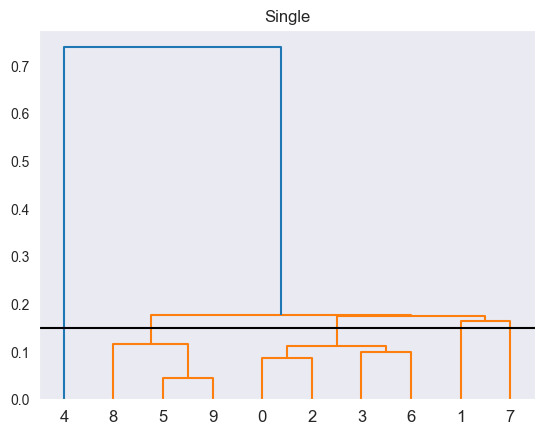
\includegraphics[width=\textwidth]{single_link_image.png}
         \end{minipage}
        \hfill
        \begin{minipage}[b]{0.48\textwidth}
            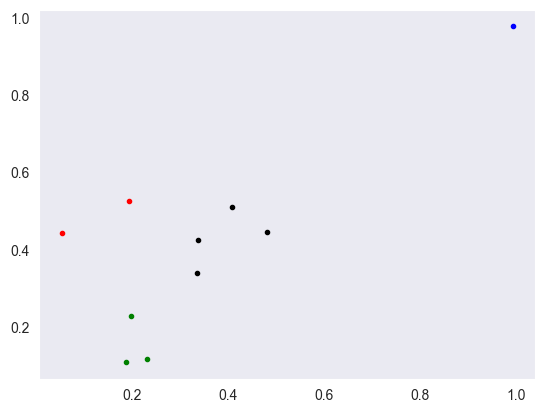
\includegraphics[width=\textwidth]{assigned_groups_single_link.png}
        \end{minipage}
    \end{figure}

 For example, in the provided image, for Single Linkage, a threshold of 0.15 produces five clusters because it intersects in five branches.
\end{frame}

\begin{frame}{Comparison of Different Linkages}
    \begin{figure}
        \centering
        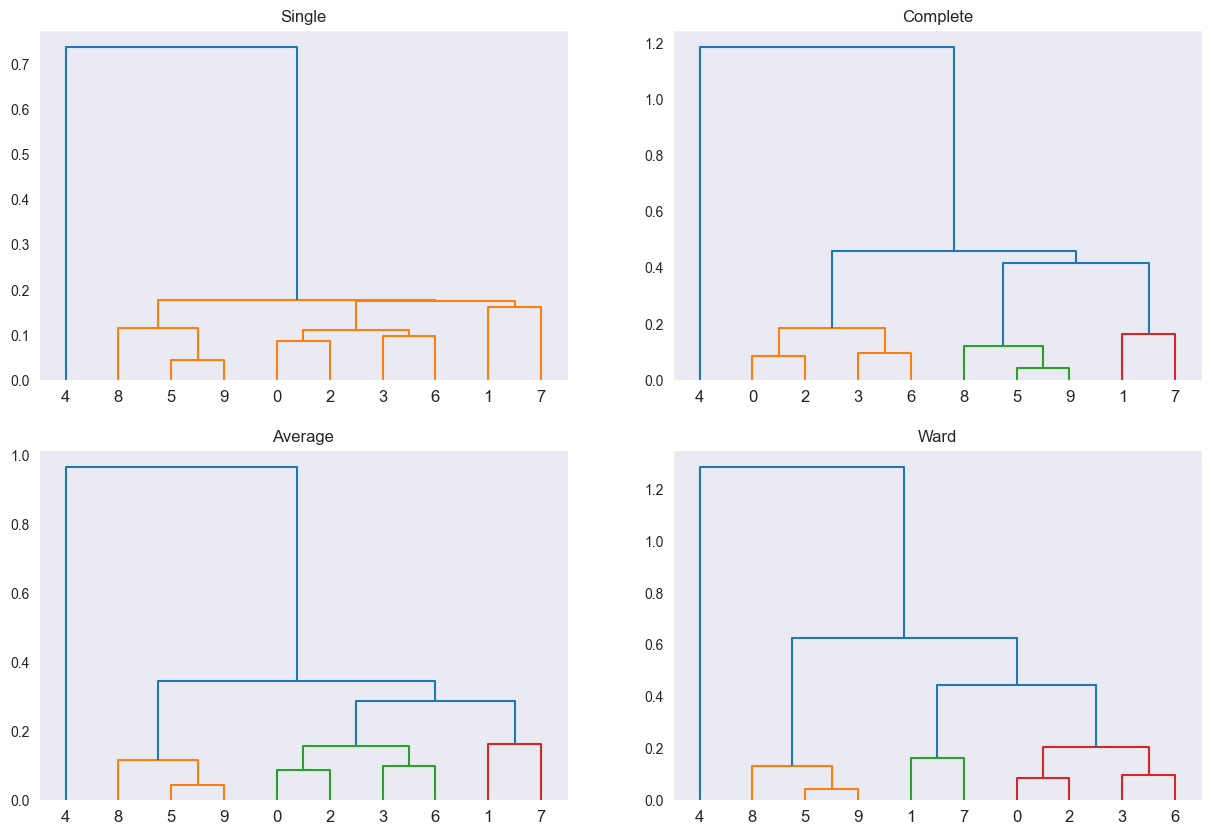
\includegraphics[scale=0.3]{different_linkages.png}
        \caption{Different linkages can produce different clusters, even with the same threshold or with same $k$.}
        \label{fig:enter-label}
    \end{figure}
\end{frame}
   
    


%\begin{frame}{Why this algorithm works}
    
%\end{frame}

\begin{frame}{Advantages of Hierarchical Clustering}
    \begin{outline}
        \1 Unlike in the $k$-means or spectral clustering algorithms, don't have to choose the number of clusters $k$ to partition into at the beginning. This is an advantage because when presented with data you may not know the true number of clusters which exist.
        \1 Provides a hierarchy of clusters.
    \end{outline}
\end{frame}

\begin{frame}{Disadvantages of Hierarchical Clustering}
    \begin{outline}
        \1 May have imbalanced clusters.
    \end{outline}
\end{frame}

\begin{frame}
\frametitle{References}
\bibliographystyle{plain}
\bibliography{refs}
\nocite{*}
\end{frame}

\end{document}